\documentclass[12pt, oneside]{book}
\usepackage{graphicx}  % this is for includegraphics

\usepackage{setspace}
\onehalfspacing % this sets spacing to 1.5 


\usepackage{amsmath}
\usepackage{amsthm} % for theorems, lemmas etc
\usepackage{amsfonts}
\usepackage{lipsum} % to generate the lipsum random text in the sample
\usepackage{tikz}
\usepackage{siunitx}

\usetikzlibrary{calc,decorations.pathmorphing,patterns}


\usepackage[colorlinks=true, urlcolor=blue, pdfborder={0 0 0}]{hyperref}
\hypersetup{
     colorlinks   = true,
     citecolor    = blue
}

\theoremstyle{plain}
\newtheorem{theorem}{Theorem}[section]
\newtheorem{proposition}[theorem]{Proposition}
\newtheorem{lemma}[theorem]{Lemma}
\newtheorem{corollary}[theorem]{Corollary}
\newtheorem{fact}[theorem]{Fact}

\theoremstyle{definition}
\newtheorem{definition}[theorem]{Definition}
\newtheorem{example}[theorem]{Example}
\newtheorem{remark}[theorem]{Remark}
\newtheorem{remarks}[theorem]{Remarks}

\newcommand{\Cov}{\mathrm{Cov}}
\newcommand{\Var}{\mathrm{Var}}

\begin{document}

\begin{titlepage}
\begin{center}
        \vspace{-2cm}
Mathematical Finance MSc Dissertation MTH775P, 2018/19 
		\\
        \Huge
        \textbf{Accelerated Grids}
        \\        
        \vspace{0.4cm}
        \LARGE
        Optimizing Solvers for Financial Partial Differential Equations
        \\        
        \vspace{0.4cm}        
        \textbf{Mustafa Berke Erdis, ID 180883925}% student name and number        
        \\
        \large Supervisor: Dr. Sebastian del Bano Rollin
        \\
        \vspace{0.9cm}
        \includegraphics[scale=0.23]{QMCrest.png}
        \\
        \vspace{0.9cm}        
        \LARGE 
        A thesis presented for the degree of\\
        Master in Sciences in \emph{Mathematical Finance}\\
        \vspace{0.7cm}        
        \Large
        School of Mathematical Sciences\\ 
        and \emph{School of Economics and Finance}\\
        Queen Mary University of London \\
    \end{center}
\end{titlepage}


\chapter*{Declaration of original work}
\begin{flushright}
This declaration is made on \today.
\end{flushright}


{\bf Student's Declaration:}
I, Mustafa Berke Erdis, hereby declare that the work in this thesis 
is my original work. I have not copied from any other students' work, work of 
mine submitted elsewhere,  or from any other sources except where due reference or acknowledgement is made explicitly in the text, nor has any part been written for me by another person.

Referenced text has been flagged by:
\begin{enumerate}
\item Using italic fonts, {\bf and} % LaTeX: {\it text}  
\item using quotation marks ``\ldots '', {\bf and}
\item explicitly mentioning the source in the text.
\end{enumerate}

%This excludes any definitions known from your modules or undethat can be found in an undergraduate text book.

\newpage

\thispagestyle{empty}
        \begin{flushright}
                This work is dedicated to my family.
        \end{flushright}
\vspace{\stretch{2}}\null



\chapter*{Acknowledgements}
Here you thank people that have helped you in the journey. \\
\lipsum[100] % replace this by your text

\chapter*{Abstract}
\begin{center}
\small 
Here you write a short summary, around 10 lines, of your work. \\
\lipsum[100]% replace this by your text
\end{center}       


\chapter*{Preface}
Here  you write a summary of the work. A paragraph on the motivation, previous work, then maybe a brief chapter by chapter summary. 

\lipsum[100]% replace this by your text



\begin{flushright}
Queen Mary University of London\\
12${}^{\text{th}}$ August 2019
\end{flushright}


\tableofcontents

\chapter{Introduction}

\section{Pricing Financial Derivatives}\label{Pricing Financial Derivatives}
\subsection{The Risk Neutral Approach}

$ S(t) = S(0) exp((\alpha - \sigma^2/2)t + \sigma B(t)) $
\subsection{Solving Financial Partial Differential Equations}

\begin{theorem}[{\cite[Theorem 2.3]{Petri}, see also \cite[pg. 45]{BlackScholes}}]\label{PetriTheorem}
The Gramm matrix for $E_8$ is:
$$
\begin{pmatrix}
2	&-1&0	&0	&0	&0	&0	&0\\
-1	&2	&-1	&0	&0	&0	&0	&0\\
0	&-1	&2	&-1	&0	&0	&0	&-1\\
0	&0	&-1	&2	&-1	&0	&0	&0\\
0	&0	&0	&-1	&2	&-1	&0	&0\\
0	&0	&0	&0	&-1	&2	&-1	&0\\
0	&0	&0	&0	&0	&-1	&2	&0\\
0	&0	&-1	&0	&0	&0	&0	&2
\end{pmatrix}.
$$
\end{theorem}

Recall the theorem of Petri \ref{PetriTheorem}
Look at section \ref{contentsofthesis}.



\section{Finite Difference Methods}
$ \frac{\partial u}{\partial t} = a(t,x) \frac{\partial^2 u}{\partial x^2} + b(t,x) \frac{\partial u}{\partial x} + c(t,x) u(t,x) + d(t,x) $

a(t,x) Diffusion coefficient
b(t,x) Convection coefficient
c(t,x) reaction coefficient
d(t,x) source coefficient

1st order Forward Difference
$ \frac{\partial u}{\partial t} = \frac{u^{n+1}_i - u^n_i}{\Delta t} $

1st order Central Difference 
$ \frac{\partial u}{\partial x} = \frac{u^{n}_{i+1} - u^n_i}{\Delta t} $

2nd order Central Difference 
$ \frac{\partial^2 u}{\partial x^2} = \frac{u^n_{i+1}- 2u^n_i + u^n_{i-1}}{(\Delta x)^2} $



\subsection{Explicit Method}
Explicit method is a forward time, central space scheme .

Explicit method can be generalized as:
$ u_j^{n+1} = \alpha u_{j-1}^{n} + \beta u_{j}^{n} + \gamma u_{j+1}^{n} $

$ r = \frac{\delta t}{\delta x^2} $

For heat equation:
$ \alpha =  r, \beta = 1 - 2r, \gamma = r $

For black-scholes equation:
$ \alpha =  \frac{\sigma^2 j^2 \Delta t}{2} - \frac{r j \Delta t}{2}, \beta = 1 - \sigma^2 j^2 \Delta t - r \Delta t, \gamma = \frac{\sigma^2 j^2 \Delta t}{2} - \frac{r j \Delta t}{2} $

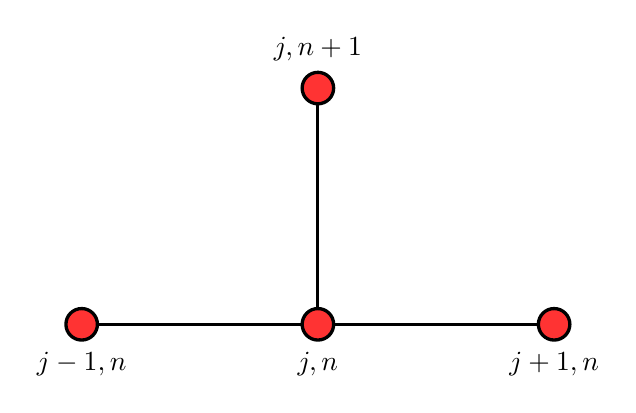
\begin{tikzpicture}[decorate]

 
 \filldraw[fill=red!80!white, draw=black,very thick] (5,5) circle (0.2cm);
 \draw[line width=0.4mm] (5,4.8) -- (5,2.2);
 \node at (5, 5.5) {$j, n+1$};
 

 \filldraw[fill=red!80!white, draw=black,very thick] (5,2) circle (0.2cm);
 \node at (5, 1.5) {$j, n$};
 \draw[line width=0.4mm] (4.8,2) -- (2.2,2);
 \filldraw[fill=red!80!white, draw=black,very thick] (2,2) circle (0.2cm);
  \node at (2, 1.5) {$j-1, n$};
 
 \draw[line width=0.4mm] (5.2,2) -- (7.8,2);
 \filldraw[fill=red!80!white, draw=black,very thick] (8,2) circle (0.2cm);
 \node at (8, 1.5) {$j+1, n$}; 
  
  
 %\draw[line width=0.4mm] (5,1.8) -- (5,-0.8);
 %\filldraw[fill=red!80!white, draw=black,very thick] (5,-1) circle (0.2cm);
 %\node at (5, -1.5) {$j, n-1$};  




 
\end{tikzpicture}

\subsection{Implicit Method}

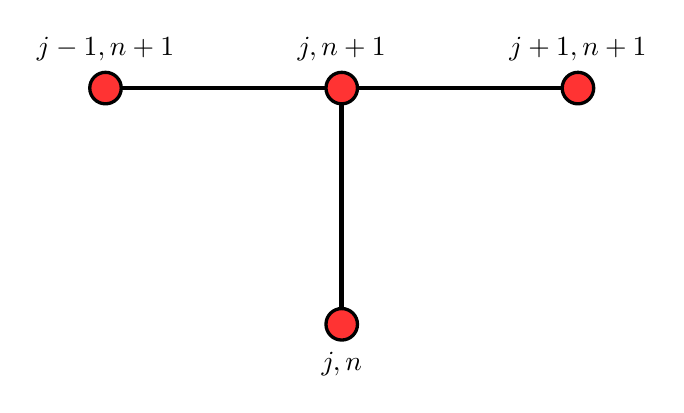
\begin{tikzpicture}[decorate]

 
 %\filldraw[fill=red!80!white, draw=black,very thick] (5,5) circle (0.2cm);
 %\draw[line width=0.4mm] (5,4.8) -- (5,2.2);
 %\node at (5, 5.5) {$j, n+1$};
 

 \filldraw[fill=red!80!white, draw=black,very thick] (5,2) circle (0.2cm);
 \node at (5, 2.5) {$j, n+1$};
 \draw[line width=0.6mm] (4.8,2) -- (2.2,2);
 \filldraw[fill=red!80!white, draw=black,very thick] (2,2) circle (0.2cm);
  \node at (2, 2.5) {$j-1, n+1$};
 
 \draw[line width=0.6mm] (5.2,2) -- (7.8,2);
 \filldraw[fill=red!80!white, draw=black,very thick] (8,2) circle (0.2cm);
 \node at (8, 2.5) {$j+1, n+1$}; 
  
  
 \draw[line width=0.6mm] (5,1.8) -- (5,-0.8);
 \filldraw[fill=red!80!white, draw=black,very thick] (5,-1) circle (0.2cm);
 \node at (5, -1.5) {$j, n$};  
 
\end{tikzpicture}

\subsection{Theta Method and Crank-Nicholson Method}

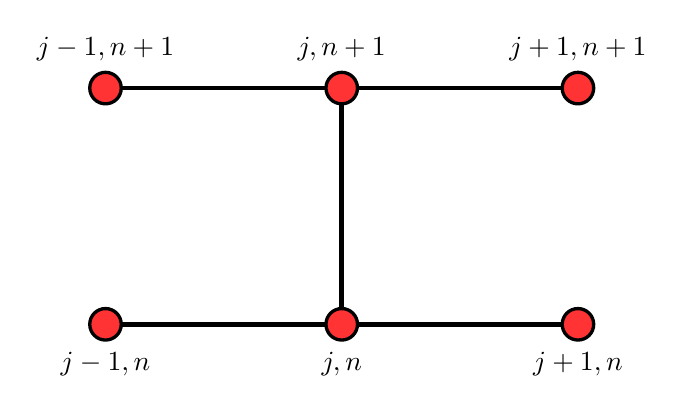
\begin{tikzpicture}[decorate]

 
 %\filldraw[fill=red!80!white, draw=black,very thick] (5,5) circle (0.2cm);
 %\draw[line width=0.4mm] (5,4.8) -- (5,2.2);
 %\node at (5, 5.5) {$j, n+1$};
 

 \filldraw[fill=red!80!white, draw=black,very thick] (5,2) circle (0.2cm);
 \node at (5, 2.5) {$j, n+1$};
 \draw[line width=0.6mm] (4.8,2) -- (2.2,2);
 \filldraw[fill=red!80!white, draw=black,very thick] (2,2) circle (0.2cm);
  \node at (2, 2.5) {$j-1, n+1$};
 
 \draw[line width=0.6mm] (5.2,2) -- (7.8,2);
 \filldraw[fill=red!80!white, draw=black,very thick] (8,2) circle (0.2cm);
 \node at (8, 2.5) {$j+1, n+1$}; 
  
  
  
 \draw[line width=0.6mm] (5,1.8) -- (5,-0.8);
 \filldraw[fill=red!80!white, draw=black,very thick] (5,-1) circle (0.2cm);
 \node at (5, -1.5) {$j, n$};  

\draw[line width=0.6mm] (4.8,-1) -- (2.2,-1);
\filldraw[fill=red!80!white, draw=black,very thick] (2,-1) circle (0.2cm);
 \node at (2, -1.5) {$j-1, n$};  

\draw[line width=0.6mm] (5.2,-1) -- (7.8,-1);
\filldraw[fill=red!80!white, draw=black,very thick] (8,-1) circle (0.2cm);
 \node at (8, -1.5) {$j+1, n$};  
 
\end{tikzpicture}

\subsection{Alternating Direction Implicit Method}

\subsection{Rannacher Trick}


\section{Optimizations}

\subsection{Compilers}
\subsection{32 bit and 64 bit}

\subsection{Optimization Switches}

\subsection{Tridiagonal Solvers}

\subsection{Threading}

\subsection{OpenMP}
\subsection{AVX and Intrinsics}
\subsection{GPGPU}
\subsection{Cloud Applications}

\chapter{Optimization of Financial Partial Differential Equations}

\section{Timing the Code}
\subsection{Windows API}

\subsection{Chrono Library}



\chapter{Conclusions}


\appendix
\chapter{Implementation of the {\tt FiniteDifferenceMethod} class}
\lipsum[100]
\chapter[shorter running title]{Additional details on the Gundermanian determinant}
\lipsum[100]



\bibliographystyle{plain}
\begin{thebibliography}{12}
\bibitem{thomas} Thomas, James W. {\it Numerical Partial Differential Equations: Finite Difference Methods.}, pp. 164, Springer, 1998.

\bibitem{klebaner}Klebaner, Fima C. {\it Introduction to Stochastic Calculus with Applications.}, pp. 155, Imperial College Press, 2005.

\bibitem{kusswurm}Kusswurm, Daniel. {\it Modern x86 Assembly Language Programming: 32-Bit, 64-Bit, SSE, and AVX.} Apress, 2015.
\bibitem[P99]{Petri}
   William Petri, 
  {\it Analysis of infinitely generated frog complexes},
	Rendicoti Ran\ae \ Analysorum, 234 {\bf (4)}, 34--21, 2015
\bibitem[Ross]{Ross}
  Sheldon Ross, {\it 
  \href{https://www-dawsonera-com.ezproxy.library.qmul.ac.uk/abstract/9781139069694}{An Elementary Introduction to Mathematical Finance}},
	3rd Edition, Cambridge University Press, 2011
	\bibitem[Hull]{Hull}
	John C. Hull, 
	{\it \href{https://www-dawsonera-com.ezproxy.library.qmul.ac.uk/abstract/9781447930419}{Options, Futures, and Other Derivatives}},
	8th Edition, Pearson Education, 2011
	\bibitem[BS]{BlackScholes}
	Fischer Black and  Myron Scholes,
	{\it \href{https://www.cs.princeton.edu/courses/archive/fall09/cos323/papers/black_scholes73.pdf}
	{The Pricing of Options and Corporate Liabilities}},
	Journal of Political Economy 81 {\bf 3}, 637--654,  (1973)
	
\end{thebibliography}



\end{document}